\documentclass[1p]{elsarticle_modified}
%\bibliographystyle{elsarticle-num}

%\usepackage[colorlinks]{hyperref}
%\usepackage{abbrmath_seonhwa} %\Abb, \Ascr, \Acal ,\Abf, \Afrak
\usepackage{amsfonts}
\usepackage{amssymb}
\usepackage{amsmath}
\usepackage{amsthm}
\usepackage{scalefnt}
\usepackage{amsbsy}
\usepackage{kotex}
\usepackage{caption}
\usepackage{subfig}
\usepackage{color}
\usepackage{graphicx}
\usepackage{xcolor} %% white, black, red, green, blue, cyan, magenta, yellow
\usepackage{float}
\usepackage{setspace}
\usepackage{hyperref}

\usepackage{tikz}
\usetikzlibrary{arrows}

\usepackage{multirow}
\usepackage{array} % fixed length table
\usepackage{hhline}

%%%%%%%%%%%%%%%%%%%%%
\makeatletter
\renewcommand*\env@matrix[1][\arraystretch]{%
	\edef\arraystretch{#1}%
	\hskip -\arraycolsep
	\let\@ifnextchar\new@ifnextchar
	\array{*\c@MaxMatrixCols c}}
\makeatother %https://tex.stackexchange.com/questions/14071/how-can-i-increase-the-line-spacing-in-a-matrix
%%%%%%%%%%%%%%%

\usepackage[normalem]{ulem}

\newcommand{\msout}[1]{\ifmmode\text{\sout{\ensuremath{#1}}}\else\sout{#1}\fi}
%SOURCE: \msout is \stkout macro in https://tex.stackexchange.com/questions/20609/strikeout-in-math-mode

\newcommand{\cancel}[1]{
	\ifmmode
	{\color{red}\msout{#1}}
	\else
	{\color{red}\sout{#1}}
	\fi
}

\newcommand{\add}[1]{
	{\color{blue}\uwave{#1}}
}

\newcommand{\replace}[2]{
	\ifmmode
	{\color{red}\msout{#1}}{\color{blue}\uwave{#2}}
	\else
	{\color{red}\sout{#1}}{\color{blue}\uwave{#2}}
	\fi
}

\newcommand{\Sol}{\mathcal{S}} %segment
\newcommand{\D}{D} %diagram
\newcommand{\A}{\mathcal{A}} %arc


%%%%%%%%%%%%%%%%%%%%%%%%%%%%%5 test

\def\sl{\operatorname{\textup{SL}}(2,\Cbb)}
\def\psl{\operatorname{\textup{PSL}}(2,\Cbb)}
\def\quan{\mkern 1mu \triangleright \mkern 1mu}

\theoremstyle{definition}
\newtheorem{thm}{Theorem}[section]
\newtheorem{prop}[thm]{Proposition}
\newtheorem{lem}[thm]{Lemma}
\newtheorem{ques}[thm]{Question}
\newtheorem{cor}[thm]{Corollary}
\newtheorem{defn}[thm]{Definition}
\newtheorem{exam}[thm]{Example}
\newtheorem{rmk}[thm]{Remark}
\newtheorem{alg}[thm]{Algorithm}

\newcommand{\I}{\sqrt{-1}}
\begin{document}

%\begin{frontmatter}
%
%\title{Boundary parabolic representations of knots up to 8 crossings}
%
%%% Group authors per affiliation:
%\author{Yunhi Cho} 
%\address{Department of Mathematics, University of Seoul, Seoul, Korea}
%\ead{yhcho@uos.ac.kr}
%
%
%\author{Seonhwa Kim} %\fnref{s_kim}}
%\address{Center for Geometry and Physics, Institute for Basic Science, Pohang, 37673, Korea}
%\ead{ryeona17@ibs.re.kr}
%
%\author{Hyuk Kim}
%\address{Department of Mathematical Sciences, Seoul National University, Seoul 08826, Korea}
%\ead{hyukkim@snu.ac.kr}
%
%\author{Seokbeom Yoon}
%\address{Department of Mathematical Sciences, Seoul National University, Seoul, 08826,  Korea}
%\ead{sbyoon15@snu.ac.kr}
%
%\begin{abstract}
%We find all boundary parabolic representation of knots up to 8 crossings.
%
%\end{abstract}
%\begin{keyword}
%    \MSC[2010] 57M25 
%\end{keyword}
%
%\end{frontmatter}

%\linenumbers
%\tableofcontents
%
\newcommand\colored[1]{\textcolor{white}{\rule[-0.35ex]{0.8em}{1.4ex}}\kern-0.8em\color{red} #1}%
%\newcommand\colored[1]{\textcolor{white}{ #1}\kern-2.17ex	\textcolor{white}{ #1}\kern-1.81ex	\textcolor{white}{ #1}\kern-2.15ex\color{red}#1	}

{\Large $\underline{11n_{93}~(K11n_{93})}$}

\setlength{\tabcolsep}{10pt}
\renewcommand{\arraystretch}{1.6}
\vspace{1cm}\begin{tabular}{m{100pt}>{\centering\arraybackslash}m{274pt}}
\multirow{5}{120pt}{
	\centering
	\includegraphics[width=112pt]{../../../GIT/diagram.site/Diagrams/png/709_11n_93.png}\\
\ \ \ A knot diagram\footnotemark}&
\allowdisplaybreaks
\textbf{Linearized knot diagam} \\
\cline{2-2}
 &
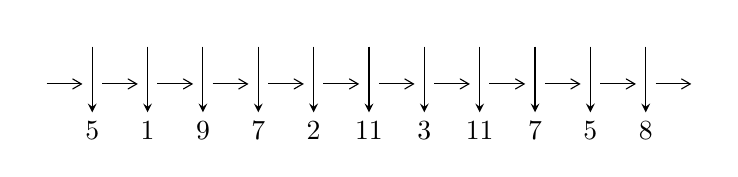
\begin{tikzpicture}[x=20pt, y=17pt]
	% nodes
	\node (C0) at (0, 0) {};
	\node (C1) at (1, 0) {};
	\node (C1U) at (1, +1) {};
	\node (C1D) at (1, -1) {5};

	\node (C2) at (2, 0) {};
	\node (C2U) at (2, +1) {};
	\node (C2D) at (2, -1) {1};

	\node (C3) at (3, 0) {};
	\node (C3U) at (3, +1) {};
	\node (C3D) at (3, -1) {9};

	\node (C4) at (4, 0) {};
	\node (C4U) at (4, +1) {};
	\node (C4D) at (4, -1) {7};

	\node (C5) at (5, 0) {};
	\node (C5U) at (5, +1) {};
	\node (C5D) at (5, -1) {2};

	\node (C6) at (6, 0) {};
	\node (C6U) at (6, +1) {};
	\node (C6D) at (6, -1) {11};

	\node (C7) at (7, 0) {};
	\node (C7U) at (7, +1) {};
	\node (C7D) at (7, -1) {3};

	\node (C8) at (8, 0) {};
	\node (C8U) at (8, +1) {};
	\node (C8D) at (8, -1) {11};

	\node (C9) at (9, 0) {};
	\node (C9U) at (9, +1) {};
	\node (C9D) at (9, -1) {7};

	\node (C10) at (10, 0) {};
	\node (C10U) at (10, +1) {};
	\node (C10D) at (10, -1) {5};

	\node (C11) at (11, 0) {};
	\node (C11U) at (11, +1) {};
	\node (C11D) at (11, -1) {8};
	\node (C12) at (12, 0) {};

	% arrows
	\draw[->,>={angle 60}]
	(C0) edge (C1) (C1) edge (C2) (C2) edge (C3) (C3) edge (C4) (C4) edge (C5) (C5) edge (C6) (C6) edge (C7) (C7) edge (C8) (C8) edge (C9) (C9) edge (C10) (C10) edge (C11) (C11) edge (C12) ;	\draw[->,>=stealth]
	(C1U) edge (C1D) (C2U) edge (C2D) (C3U) edge (C3D) (C4U) edge (C4D) (C5U) edge (C5D) (C6U) edge (C6D) (C7U) edge (C7D) (C8U) edge (C8D) (C9U) edge (C9D) (C10U) edge (C10D) (C11U) edge (C11D) ;
	\end{tikzpicture} \\
\hhline{~~} \\& 
\textbf{Solving Sequence} \\ \cline{2-2} 
 &
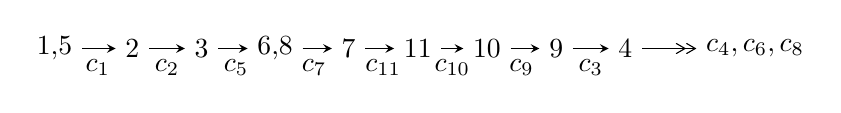
\begin{tikzpicture}[x=25pt, y=7pt]
	% node
	\node (A0) at (-1/8, 0) {1,5};
	\node (A1) at (1, 0) {2};
	\node (A2) at (2, 0) {3};
	\node (A3) at (49/16, 0) {6,8};
	\node (A4) at (33/8, 0) {7};
	\node (A5) at (41/8, 0) {11};
	\node (A6) at (49/8, 0) {10};
	\node (A7) at (57/8, 0) {9};
	\node (A8) at (65/8, 0) {4};
	\node (C1) at (1/2, -1) {$c_{1}$};
	\node (C2) at (3/2, -1) {$c_{2}$};
	\node (C3) at (5/2, -1) {$c_{5}$};
	\node (C4) at (29/8, -1) {$c_{7}$};
	\node (C5) at (37/8, -1) {$c_{11}$};
	\node (C6) at (45/8, -1) {$c_{10}$};
	\node (C7) at (53/8, -1) {$c_{9}$};
	\node (C8) at (61/8, -1) {$c_{3}$};
	\node (A9) at (10, 0) {$c_{4},c_{6},c_{8}$};

	% edge
	\draw[->,>=stealth]	
	(A0) edge (A1) (A1) edge (A2) (A2) edge (A3) (A3) edge (A4) (A4) edge (A5) (A5) edge (A6) (A6) edge (A7) (A7) edge (A8) ;
	\draw[->>,>={angle 60}]	
	(A8) edge (A9);
\end{tikzpicture} \\ 

\end{tabular} \\

\footnotetext{
The image of knot diagram is generated by the software ``\textbf{Draw programme}" developed by Andrew Bartholomew(\url{http://www.layer8.co.uk/maths/draw/index.htm\#Running-draw}), where we modified some parts for our purpose(\url{https://github.com/CATsTAILs/LinksPainter}).
}\phantom \\ \newline 
\centering \textbf{Ideals for irreducible components\footnotemark of $X_{\text{par}}$} 
 
\begin{align*}
I^u_{1}&=\langle 
-1.36953\times10^{20} u^{33}-1.71275\times10^{20} u^{32}+\cdots+2.52092\times10^{19} b+1.79272\times10^{20},\\
\phantom{I^u_{1}}&\phantom{= \langle  }2.14966\times10^{20} u^{33}+2.97471\times10^{20} u^{32}+\cdots+2.52092\times10^{19} a-2.61593\times10^{20},\;u^{34}+2 u^{33}+\cdots-3 u-1\rangle \\
I^u_{2}&=\langle 
u^{10}-3 u^8+u^7+5 u^6- u^5-5 u^4+2 u^3+3 u^2+b-1,\\
\phantom{I^u_{2}}&\phantom{= \langle  }3 u^{10}+2 u^9-9 u^8-6 u^7+15 u^6+13 u^5-13 u^4-9 u^3+6 u^2+a+5 u-4,\\
\phantom{I^u_{2}}&\phantom{= \langle  }u^{11}+u^{10}-3 u^9-3 u^8+5 u^7+6 u^6-4 u^5-5 u^4+2 u^3+3 u^2- u-1\rangle \\
\\
\end{align*}
\raggedright * 2 irreducible components of $\dim_{\mathbb{C}}=0$, with total 45 representations.\\
\footnotetext{All coefficients of polynomials are rational numbers. But the coefficients are sometimes approximated in decimal forms when there is not enough margin.}
\newpage
\renewcommand{\arraystretch}{1}
\centering \section*{I. $I^u_{1}= \langle -1.37\times10^{20} u^{33}-1.71\times10^{20} u^{32}+\cdots+2.52\times10^{19} b+1.79\times10^{20},\;2.15\times10^{20} u^{33}+2.97\times10^{20} u^{32}+\cdots+2.52\times10^{19} a-2.62\times10^{20},\;u^{34}+2 u^{33}+\cdots-3 u-1 \rangle$}
\flushleft \textbf{(i) Arc colorings}\\
\begin{tabular}{m{7pt} m{180pt} m{7pt} m{180pt} }
\flushright $a_{1}=$&$\begin{pmatrix}1\\0\end{pmatrix}$ \\
\flushright $a_{5}=$&$\begin{pmatrix}0\\u\end{pmatrix}$ \\
\flushright $a_{2}=$&$\begin{pmatrix}1\\u^2\end{pmatrix}$ \\
\flushright $a_{3}=$&$\begin{pmatrix}- u^2+1\\u^2\end{pmatrix}$ \\
\flushright $a_{6}=$&$\begin{pmatrix}- u\\- u^3+u\end{pmatrix}$ \\
\flushright $a_{8}=$&$\begin{pmatrix}-8.52729 u^{33}-11.8001 u^{32}+\cdots+4.46895 u+10.3769\\5.43266 u^{33}+6.79414 u^{32}+\cdots-10.8889 u-7.11138\end{pmatrix}$ \\
\flushright $a_{7}=$&$\begin{pmatrix}-5.44195 u^{33}-7.75886 u^{32}+\cdots-0.159734 u+6.36806\\8.48937 u^{33}+10.7511 u^{32}+\cdots-17.6044 u-11.3972\end{pmatrix}$ \\
\flushright $a_{11}=$&$\begin{pmatrix}0.678159 u^{33}+0.639889 u^{32}+\cdots+4.60728 u+2.39805\\4.96030 u^{33}+6.55238 u^{32}+\cdots-11.3046 u-7.35481\end{pmatrix}$ \\
\flushright $a_{10}=$&$\begin{pmatrix}0.678159 u^{33}+0.639889 u^{32}+\cdots+4.60728 u+2.39805\\3.98582 u^{33}+5.46449 u^{32}+\cdots-9.83347 u-6.63838\end{pmatrix}$ \\
\flushright $a_{9}=$&$\begin{pmatrix}0.605729 u^{33}-0.505670 u^{32}+\cdots-20.5146 u-2.20921\\-0.341296 u^{33}+0.0744426 u^{32}+\cdots+1.81668 u-0.281935\end{pmatrix}$ \\
\flushright $a_{4}=$&$\begin{pmatrix}4.14625 u^{33}+3.90637 u^{32}+\cdots-34.9982 u-9.83659\\-4.60795 u^{33}-5.18060 u^{32}+\cdots+10.8857 u+5.66173\end{pmatrix}$\\ \flushright $a_{4}=$&$\begin{pmatrix}4.14625 u^{33}+3.90637 u^{32}+\cdots-34.9982 u-9.83659\\-4.60795 u^{33}-5.18060 u^{32}+\cdots+10.8857 u+5.66173\end{pmatrix}$\\&\end{tabular}
\flushleft \textbf{(ii) Obstruction class $= -1$}\\~\\
\flushleft \textbf{(iii) Cusp Shapes $= -\frac{45272021734023345182}{25209200843466515639} u^{33}-\frac{27918280350195858852}{25209200843466515639} u^{32}+\cdots+\frac{482980842236749416852}{25209200843466515639} u-\frac{268074501698973471381}{25209200843466515639}$}\\~\\
\newpage\renewcommand{\arraystretch}{1}
\flushleft \textbf{(iv) u-Polynomials at the component}\newline \\
\begin{tabular}{m{50pt}|m{274pt}}
Crossings & \hspace{64pt}u-Polynomials at each crossing \\
\hline $$\begin{aligned}c_{1},c_{5}\end{aligned}$$&$\begin{aligned}
&u^{34}+2 u^{33}+\cdots-3 u-1
\end{aligned}$\\
\hline $$\begin{aligned}c_{2}\end{aligned}$$&$\begin{aligned}
&u^{34}+20 u^{33}+\cdots+23 u+1
\end{aligned}$\\
\hline $$\begin{aligned}c_{3},c_{10}\end{aligned}$$&$\begin{aligned}
&u^{34}- u^{33}+\cdots+10 u-1
\end{aligned}$\\
\hline $$\begin{aligned}c_{4}\end{aligned}$$&$\begin{aligned}
&u^{34}-3 u^{33}+\cdots+16 u+1
\end{aligned}$\\
\hline $$\begin{aligned}c_{6}\end{aligned}$$&$\begin{aligned}
&u^{34}+2 u^{33}+\cdots-2561 u-1007
\end{aligned}$\\
\hline $$\begin{aligned}c_{7}\end{aligned}$$&$\begin{aligned}
&u^{34}+u^{33}+\cdots-36 u-9
\end{aligned}$\\
\hline $$\begin{aligned}c_{8},c_{11}\end{aligned}$$&$\begin{aligned}
&u^{34}-4 u^{33}+\cdots+5 u-7
\end{aligned}$\\
\hline $$\begin{aligned}c_{9}\end{aligned}$$&$\begin{aligned}
&u^{34}-2 u^{33}+\cdots-415 u+31
\end{aligned}$\\
\hline
\end{tabular}\\~\\
\newpage\renewcommand{\arraystretch}{1}
\flushleft \textbf{(v) Riley Polynomials at the component}\newline \\
\begin{tabular}{m{50pt}|m{274pt}}
Crossings & \hspace{64pt}Riley Polynomials at each crossing \\
\hline $$\begin{aligned}c_{1},c_{5}\end{aligned}$$&$\begin{aligned}
&y^{34}-20 y^{33}+\cdots-23 y+1
\end{aligned}$\\
\hline $$\begin{aligned}c_{2}\end{aligned}$$&$\begin{aligned}
&y^{34}-4 y^{33}+\cdots-215 y+1
\end{aligned}$\\
\hline $$\begin{aligned}c_{3},c_{10}\end{aligned}$$&$\begin{aligned}
&y^{34}-45 y^{33}+\cdots+54 y+1
\end{aligned}$\\
\hline $$\begin{aligned}c_{4}\end{aligned}$$&$\begin{aligned}
&y^{34}-61 y^{33}+\cdots+4 y+1
\end{aligned}$\\
\hline $$\begin{aligned}c_{6}\end{aligned}$$&$\begin{aligned}
&y^{34}-48 y^{33}+\cdots-16050703 y+1014049
\end{aligned}$\\
\hline $$\begin{aligned}c_{7}\end{aligned}$$&$\begin{aligned}
&y^{34}+11 y^{33}+\cdots-576 y+81
\end{aligned}$\\
\hline $$\begin{aligned}c_{8},c_{11}\end{aligned}$$&$\begin{aligned}
&y^{34}+12 y^{33}+\cdots-375 y+49
\end{aligned}$\\
\hline $$\begin{aligned}c_{9}\end{aligned}$$&$\begin{aligned}
&y^{34}-48 y^{33}+\cdots-50333 y+961
\end{aligned}$\\
\hline
\end{tabular}\\~\\
\newpage\flushleft \textbf{(vi) Complex Volumes and Cusp Shapes}
$$\begin{array}{c|c|c}  
\text{Solutions to }I^u_{1}& \I (\text{vol} + \sqrt{-1}CS) & \text{Cusp shape}\\
 \hline 
\begin{aligned}
u &= \phantom{-}0.977418 + 0.219996 I \\
a &= -0.444506 + 0.228131 I \\
b &= -1.177060 + 0.358042 I\end{aligned}
 & -3.42083 - 0.72607 I & -14.2661 + 6.0469 I \\ \hline\begin{aligned}
u &= \phantom{-}0.977418 - 0.219996 I \\
a &= -0.444506 - 0.228131 I \\
b &= -1.177060 - 0.358042 I\end{aligned}
 & -3.42083 + 0.72607 I & -14.2661 - 6.0469 I \\ \hline\begin{aligned}
u &= \phantom{-}0.573841 + 0.727686 I \\
a &= \phantom{-}0.107760 + 0.779562 I \\
b &= \phantom{-}0.238183 - 0.951299 I\end{aligned}
 & \phantom{-}3.89256 - 0.89641 I & -5.46445 + 2.96652 I \\ \hline\begin{aligned}
u &= \phantom{-}0.573841 - 0.727686 I \\
a &= \phantom{-}0.107760 - 0.779562 I \\
b &= \phantom{-}0.238183 + 0.951299 I\end{aligned}
 & \phantom{-}3.89256 + 0.89641 I & -5.46445 - 2.96652 I \\ \hline\begin{aligned}
u &= -1.000090 + 0.396450 I \\
a &= \phantom{-}0.995356 + 0.586804 I \\
b &= \phantom{-}0.091298 - 0.895598 I\end{aligned}
 & -0.300266 + 0.779117 I & -12.61952 - 0.14976 I \\ \hline\begin{aligned}
u &= -1.000090 - 0.396450 I \\
a &= \phantom{-}0.995356 - 0.586804 I \\
b &= \phantom{-}0.091298 + 0.895598 I\end{aligned}
 & -0.300266 - 0.779117 I & -12.61952 + 0.14976 I \\ \hline\begin{aligned}
u &= -0.878110 + 0.672399 I \\
a &= \phantom{-}0.639488 + 0.722914 I \\
b &= -0.282345 - 0.793763 I\end{aligned}
 & -0.041134 + 0.639337 I & -11.81438 + 0.98279 I \\ \hline\begin{aligned}
u &= -0.878110 - 0.672399 I \\
a &= \phantom{-}0.639488 - 0.722914 I \\
b &= -0.282345 + 0.793763 I\end{aligned}
 & -0.041134 - 0.639337 I & -11.81438 - 0.98279 I \\ \hline\begin{aligned}
u &= -0.300493 + 1.118760 I \\
a &= -0.628604 - 1.104010 I \\
b &= \phantom{-}0.708856 + 1.113100 I\end{aligned}
 & -5.84181 - 6.21635 I & -10.71032 + 3.59890 I \\ \hline\begin{aligned}
u &= -0.300493 - 1.118760 I \\
a &= -0.628604 + 1.104010 I \\
b &= \phantom{-}0.708856 - 1.113100 I\end{aligned}
 & -5.84181 + 6.21635 I & -10.71032 - 3.59890 I\\
 \hline 
 \end{array}$$\newpage$$\begin{array}{c|c|c}  
\text{Solutions to }I^u_{1}& \I (\text{vol} + \sqrt{-1}CS) & \text{Cusp shape}\\
 \hline 
\begin{aligned}
u &= -0.953057 + 0.668360 I \\
a &= -0.53608 - 1.54146 I \\
b &= -0.645636 + 0.835280 I\end{aligned}
 & -0.43138 + 4.55558 I & -13.3660 - 5.8441 I \\ \hline\begin{aligned}
u &= -0.953057 - 0.668360 I \\
a &= -0.53608 + 1.54146 I \\
b &= -0.645636 - 0.835280 I\end{aligned}
 & -0.43138 - 4.55558 I & -13.3660 + 5.8441 I \\ \hline\begin{aligned}
u &= \phantom{-}1.031700 + 0.655009 I \\
a &= \phantom{-}0.830682 - 0.780653 I \\
b &= \phantom{-}0.594629 + 0.693125 I\end{aligned}
 & \phantom{-}2.55533 - 4.41329 I & -7.45627 + 1.89093 I \\ \hline\begin{aligned}
u &= \phantom{-}1.031700 - 0.655009 I \\
a &= \phantom{-}0.830682 + 0.780653 I \\
b &= \phantom{-}0.594629 - 0.693125 I\end{aligned}
 & \phantom{-}2.55533 + 4.41329 I & -7.45627 - 1.89093 I \\ \hline\begin{aligned}
u &= -1.192910 + 0.280924 I \\
a &= -0.484338 + 0.191067 I \\
b &= -0.644248 + 0.614710 I\end{aligned}
 & -0.99260 + 2.94608 I & -14.2242 - 4.1884 I \\ \hline\begin{aligned}
u &= -1.192910 - 0.280924 I \\
a &= -0.484338 - 0.191067 I \\
b &= -0.644248 - 0.614710 I\end{aligned}
 & -0.99260 - 2.94608 I & -14.2242 + 4.1884 I \\ \hline\begin{aligned}
u &= \phantom{-}1.163230 + 0.443799 I \\
a &= \phantom{-}0.54848 - 1.89291 I \\
b &= \phantom{-}0.592978 + 1.071570 I\end{aligned}
 & -10.91160 - 3.58899 I & -13.7786 + 3.7180 I \\ \hline\begin{aligned}
u &= \phantom{-}1.163230 - 0.443799 I \\
a &= \phantom{-}0.54848 + 1.89291 I \\
b &= \phantom{-}0.592978 - 1.071570 I\end{aligned}
 & -10.91160 + 3.58899 I & -13.7786 - 3.7180 I \\ \hline\begin{aligned}
u &= -0.739045 + 0.052216 I \\
a &= -0.93579 - 1.67559 I \\
b &= -0.394062 + 1.339380 I\end{aligned}
 & \phantom{-}1.56826 + 1.68408 I & -13.99827 - 0.91587 I \\ \hline\begin{aligned}
u &= -0.739045 - 0.052216 I \\
a &= -0.93579 + 1.67559 I \\
b &= -0.394062 - 1.339380 I\end{aligned}
 & \phantom{-}1.56826 - 1.68408 I & -13.99827 + 0.91587 I\\
 \hline 
 \end{array}$$\newpage$$\begin{array}{c|c|c}  
\text{Solutions to }I^u_{1}& \I (\text{vol} + \sqrt{-1}CS) & \text{Cusp shape}\\
 \hline 
\begin{aligned}
u &= -1.162070 + 0.498975 I \\
a &= -0.258485 - 0.047341 I \\
b &= \phantom{-}1.31485 + 0.79996 I\end{aligned}
 & -10.50350 + 4.65202 I & -13.9876 - 3.4886 I \\ \hline\begin{aligned}
u &= -1.162070 - 0.498975 I \\
a &= -0.258485 + 0.047341 I \\
b &= \phantom{-}1.31485 - 0.79996 I\end{aligned}
 & -10.50350 - 4.65202 I & -13.9876 + 3.4886 I \\ \hline\begin{aligned}
u &= \phantom{-}1.183220 + 0.495063 I \\
a &= -0.910271 + 1.014240 I \\
b &= -0.63178 - 1.27610 I\end{aligned}
 & -0.32497 - 7.07104 I & -12.7900 + 6.5034 I \\ \hline\begin{aligned}
u &= \phantom{-}1.183220 - 0.495063 I \\
a &= -0.910271 - 1.014240 I \\
b &= -0.63178 + 1.27610 I\end{aligned}
 & -0.32497 + 7.07104 I & -12.7900 - 6.5034 I \\ \hline\begin{aligned}
u &= \phantom{-}0.182031 + 0.670224 I \\
a &= \phantom{-}0.59393 - 1.62022 I \\
b &= -0.306134 + 1.218490 I\end{aligned}
 & \phantom{-}2.61338 + 2.54071 I & -8.06134 - 4.21753 I \\ \hline\begin{aligned}
u &= \phantom{-}0.182031 - 0.670224 I \\
a &= \phantom{-}0.59393 + 1.62022 I \\
b &= -0.306134 - 1.218490 I\end{aligned}
 & \phantom{-}2.61338 - 2.54071 I & -8.06134 + 4.21753 I \\ \hline\begin{aligned}
u &= -0.158687 + 0.575572 I \\
a &= \phantom{-}0.27697 + 2.86042 I \\
b &= \phantom{-}0.950893 - 0.442875 I\end{aligned}
 & -7.71465 - 0.24390 I & -10.88322 - 1.02866 I \\ \hline\begin{aligned}
u &= -0.158687 - 0.575572 I \\
a &= \phantom{-}0.27697 - 2.86042 I \\
b &= \phantom{-}0.950893 + 0.442875 I\end{aligned}
 & -7.71465 + 0.24390 I & -10.88322 + 1.02866 I \\ \hline\begin{aligned}
u &= -1.27133 + 0.67164 I \\
a &= \phantom{-}0.65445 + 1.29088 I \\
b &= \phantom{-}0.91249 - 1.24105 I\end{aligned}
 & -8.8655 + 12.5839 I & -13.0129 - 6.3971 I \\ \hline\begin{aligned}
u &= -1.27133 - 0.67164 I \\
a &= \phantom{-}0.65445 - 1.29088 I \\
b &= \phantom{-}0.91249 + 1.24105 I\end{aligned}
 & -8.8655 - 12.5839 I & -13.0129 + 6.3971 I\\
 \hline 
 \end{array}$$\newpage$$\begin{array}{c|c|c}  
\text{Solutions to }I^u_{1}& \I (\text{vol} + \sqrt{-1}CS) & \text{Cusp shape}\\
 \hline 
\begin{aligned}
u &= \phantom{-}1.55789 + 0.27506 I \\
a &= -0.265249 - 0.006903 I \\
b &= \phantom{-}0.571671 - 0.692974 I\end{aligned}
 & -12.18800 + 1.09324 I & -11.00000 - 4.94776 I \\ \hline\begin{aligned}
u &= \phantom{-}1.55789 - 0.27506 I \\
a &= -0.265249 + 0.006903 I \\
b &= \phantom{-}0.571671 + 0.692974 I\end{aligned}
 & -12.18800 - 1.09324 I & -11.00000 + 4.94776 I \\ \hline\begin{aligned}
u &= -0.331451\phantom{ +0.000000I} \\
a &= \phantom{-}1.15110\phantom{ +0.000000I} \\
b &= -0.282626\phantom{ +0.000000I}\end{aligned}
 & -0.627282\phantom{ +0.000000I} & -15.7510\phantom{ +0.000000I} \\ \hline\begin{aligned}
u &= \phantom{-}0.304363\phantom{ +0.000000I} \\
a &= -8.51870\phantom{ +0.000000I} \\
b &= \phantom{-}0.493445\phantom{ +0.000000I}\end{aligned}
 & -7.76994\phantom{ +0.000000I} & -5.58750\phantom{ +0.000000I}\\
 \hline 
 \end{array}$$\newpage\newpage\renewcommand{\arraystretch}{1}
\centering \section*{II. $I^u_{2}= \langle u^{10}-3 u^8+\cdots+b-1,\;3 u^{10}+2 u^9+\cdots+a-4,\;u^{11}+u^{10}+\cdots- u-1 \rangle$}
\flushleft \textbf{(i) Arc colorings}\\
\begin{tabular}{m{7pt} m{180pt} m{7pt} m{180pt} }
\flushright $a_{1}=$&$\begin{pmatrix}1\\0\end{pmatrix}$ \\
\flushright $a_{5}=$&$\begin{pmatrix}0\\u\end{pmatrix}$ \\
\flushright $a_{2}=$&$\begin{pmatrix}1\\u^2\end{pmatrix}$ \\
\flushright $a_{3}=$&$\begin{pmatrix}- u^2+1\\u^2\end{pmatrix}$ \\
\flushright $a_{6}=$&$\begin{pmatrix}- u\\- u^3+u\end{pmatrix}$ \\
\flushright $a_{8}=$&$\begin{pmatrix}-3 u^{10}-2 u^9+9 u^8+6 u^7-15 u^6-13 u^5+13 u^4+9 u^3-6 u^2-5 u+4\\- u^{10}+3 u^8- u^7-5 u^6+u^5+5 u^4-2 u^3-3 u^2+1\end{pmatrix}$ \\
\flushright $a_{7}=$&$\begin{pmatrix}-2 u^{10}- u^9+6 u^8+3 u^7-10 u^6-7 u^5+9 u^4+5 u^3-4 u^2-4 u+3\\- u^{10}+3 u^8- u^7-5 u^6+u^5+5 u^4-3 u^3-3 u^2+u+1\end{pmatrix}$ \\
\flushright $a_{11}=$&$\begin{pmatrix}2 u^{10}+u^9-6 u^8-2 u^7+10 u^6+4 u^5-9 u^4- u^3+5 u^2+u-3\\- u^8- u^7+3 u^6+2 u^5-5 u^4-3 u^3+3 u^2+u-1\end{pmatrix}$ \\
\flushright $a_{10}=$&$\begin{pmatrix}2 u^{10}+u^9-6 u^8-2 u^7+10 u^6+4 u^5-9 u^4- u^3+5 u^2+u-3\\- u^{10}- u^9+2 u^8+2 u^7-2 u^6-3 u^5- u^4+u^2\end{pmatrix}$ \\
\flushright $a_{9}=$&$\begin{pmatrix}-4 u^{10}-2 u^9+\cdots-6 u+7\\- u^{10}- u^9+2 u^8+2 u^7-2 u^6-4 u^5- u^4+2 u^3+u^2-2 u\end{pmatrix}$ \\
\flushright $a_{4}=$&$\begin{pmatrix}6 u^{10}+2 u^9-19 u^8-5 u^7+32 u^6+14 u^5-31 u^4-8 u^3+15 u^2+7 u-9\\2 u^{10}+u^9-7 u^8-2 u^7+13 u^6+4 u^5-13 u^4-2 u^3+9 u^2+u-3\end{pmatrix}$\\ \flushright $a_{4}=$&$\begin{pmatrix}6 u^{10}+2 u^9-19 u^8-5 u^7+32 u^6+14 u^5-31 u^4-8 u^3+15 u^2+7 u-9\\2 u^{10}+u^9-7 u^8-2 u^7+13 u^6+4 u^5-13 u^4-2 u^3+9 u^2+u-3\end{pmatrix}$\\&\end{tabular}
\flushleft \textbf{(ii) Obstruction class $= 1$}\\~\\
\flushleft \textbf{(iii) Cusp Shapes $= 10 u^{10}+2 u^9-35 u^8-4 u^7+63 u^6+16 u^5-67 u^4-11 u^3+40 u^2+11 u-30$}\\~\\
\newpage\renewcommand{\arraystretch}{1}
\flushleft \textbf{(iv) u-Polynomials at the component}\newline \\
\begin{tabular}{m{50pt}|m{274pt}}
Crossings & \hspace{64pt}u-Polynomials at each crossing \\
\hline $$\begin{aligned}c_{1}\end{aligned}$$&$\begin{aligned}
&u^{11}+u^{10}-3 u^9-3 u^8+5 u^7+6 u^6-4 u^5-5 u^4+2 u^3+3 u^2- u-1
\end{aligned}$\\
\hline $$\begin{aligned}c_{2}\end{aligned}$$&$\begin{aligned}
&u^{11}+7 u^{10}+\cdots+7 u+1
\end{aligned}$\\
\hline $$\begin{aligned}c_{3}\end{aligned}$$&$\begin{aligned}
&u^{11}-6 u^9- u^8+14 u^7+3 u^6-18 u^5-4 u^4+12 u^3+3 u^2-4 u-1
\end{aligned}$\\
\hline $$\begin{aligned}c_{4}\end{aligned}$$&$\begin{aligned}
&u^{11}-4 u^{10}+\cdots-10 u+1
\end{aligned}$\\
\hline $$\begin{aligned}c_{5}\end{aligned}$$&$\begin{aligned}
&u^{11}- u^{10}-3 u^9+3 u^8+5 u^7-6 u^6-4 u^5+5 u^4+2 u^3-3 u^2- u+1
\end{aligned}$\\
\hline $$\begin{aligned}c_{6}\end{aligned}$$&$\begin{aligned}
&u^{11}+u^{10}- u^9+4 u^8-4 u^7+u^6+4 u^5-9 u^4+9 u^3-7 u^2+3 u-1
\end{aligned}$\\
\hline $$\begin{aligned}c_{7}\end{aligned}$$&$\begin{aligned}
&u^{11}+4 u^9- u^8+5 u^7-3 u^6-3 u^4-5 u^3-2 u^2-4 u-1
\end{aligned}$\\
\hline $$\begin{aligned}c_{8}\end{aligned}$$&$\begin{aligned}
&u^{11}-3 u^{10}+7 u^9-9 u^8+9 u^7-4 u^6- u^5+4 u^4-4 u^3+u^2- u-1
\end{aligned}$\\
\hline $$\begin{aligned}c_{9}\end{aligned}$$&$\begin{aligned}
&u^{11}+3 u^{10}+u^9+3 u^7+u^5- u^4- u^3+2 u^2- u+1
\end{aligned}$\\
\hline $$\begin{aligned}c_{10}\end{aligned}$$&$\begin{aligned}
&u^{11}-6 u^9+u^8+14 u^7-3 u^6-18 u^5+4 u^4+12 u^3-3 u^2-4 u+1
\end{aligned}$\\
\hline $$\begin{aligned}c_{11}\end{aligned}$$&$\begin{aligned}
&u^{11}+3 u^{10}+7 u^9+9 u^8+9 u^7+4 u^6- u^5-4 u^4-4 u^3- u^2- u+1
\end{aligned}$\\
\hline
\end{tabular}\\~\\
\newpage\renewcommand{\arraystretch}{1}
\flushleft \textbf{(v) Riley Polynomials at the component}\newline \\
\begin{tabular}{m{50pt}|m{274pt}}
Crossings & \hspace{64pt}Riley Polynomials at each crossing \\
\hline $$\begin{aligned}c_{1},c_{5}\end{aligned}$$&$\begin{aligned}
&y^{11}-7 y^{10}+\cdots+7 y-1
\end{aligned}$\\
\hline $$\begin{aligned}c_{2}\end{aligned}$$&$\begin{aligned}
&y^{11}+y^{10}+\cdots+3 y-1
\end{aligned}$\\
\hline $$\begin{aligned}c_{3},c_{10}\end{aligned}$$&$\begin{aligned}
&y^{11}-12 y^{10}+\cdots+22 y-1
\end{aligned}$\\
\hline $$\begin{aligned}c_{4}\end{aligned}$$&$\begin{aligned}
&y^{11}-4 y^{10}+\cdots+16 y-1
\end{aligned}$\\
\hline $$\begin{aligned}c_{6}\end{aligned}$$&$\begin{aligned}
&y^{11}-3 y^{10}+\cdots-5 y-1
\end{aligned}$\\
\hline $$\begin{aligned}c_{7}\end{aligned}$$&$\begin{aligned}
&y^{11}+8 y^{10}+\cdots+12 y-1
\end{aligned}$\\
\hline $$\begin{aligned}c_{8},c_{11}\end{aligned}$$&$\begin{aligned}
&y^{11}+5 y^{10}+\cdots+3 y-1
\end{aligned}$\\
\hline $$\begin{aligned}c_{9}\end{aligned}$$&$\begin{aligned}
&y^{11}-7 y^{10}+7 y^9+8 y^8+15 y^7-10 y^6-13 y^5-9 y^4+3 y^3-3 y-1
\end{aligned}$\\
\hline
\end{tabular}\\~\\
\newpage\flushleft \textbf{(vi) Complex Volumes and Cusp Shapes}
$$\begin{array}{c|c|c}  
\text{Solutions to }I^u_{2}& \I (\text{vol} + \sqrt{-1}CS) & \text{Cusp shape}\\
 \hline 
\begin{aligned}
u &= -0.699469 + 0.611146 I \\
a &= \phantom{-}0.428957 + 0.652621 I \\
b &= -0.620153 - 1.221950 I\end{aligned}
 & \phantom{-}3.01958 - 0.56743 I & -9.71824 - 0.39336 I \\ \hline\begin{aligned}
u &= -0.699469 - 0.611146 I \\
a &= \phantom{-}0.428957 - 0.652621 I \\
b &= -0.620153 + 1.221950 I\end{aligned}
 & \phantom{-}3.01958 + 0.56743 I & -9.71824 + 0.39336 I \\ \hline\begin{aligned}
u &= \phantom{-}0.875804\phantom{ +0.000000I} \\
a &= -0.670673\phantom{ +0.000000I} \\
b &= -1.06635\phantom{ +0.000000I}\end{aligned}
 & -3.03217\phantom{ +0.000000I} & -10.2530\phantom{ +0.000000I} \\ \hline\begin{aligned}
u &= -1.006850 + 0.637757 I \\
a &= -0.820799 - 1.074540 I \\
b &= -0.831904 + 0.975863 I\end{aligned}
 & \phantom{-}2.01933 + 5.51593 I & -10.60882 - 6.86396 I \\ \hline\begin{aligned}
u &= -1.006850 - 0.637757 I \\
a &= -0.820799 + 1.074540 I \\
b &= -0.831904 - 0.975863 I\end{aligned}
 & \phantom{-}2.01933 - 5.51593 I & -10.60882 + 6.86396 I \\ \hline\begin{aligned}
u &= \phantom{-}0.626035 + 0.508829 I \\
a &= \phantom{-}0.12930 + 1.93949 I \\
b &= -0.138001 - 1.197500 I\end{aligned}
 & \phantom{-}2.51249 - 2.42581 I & -7.49749 + 5.02500 I \\ \hline\begin{aligned}
u &= \phantom{-}0.626035 - 0.508829 I \\
a &= \phantom{-}0.12930 - 1.93949 I \\
b &= -0.138001 + 1.197500 I\end{aligned}
 & \phantom{-}2.51249 + 2.42581 I & -7.49749 - 5.02500 I \\ \hline\begin{aligned}
u &= \phantom{-}1.163860 + 0.576096 I \\
a &= \phantom{-}0.961303 - 0.429407 I \\
b &= \phantom{-}0.036813 + 0.809877 I\end{aligned}
 & \phantom{-}0.66663 - 2.01787 I & -8.86455 + 3.07109 I \\ \hline\begin{aligned}
u &= \phantom{-}1.163860 - 0.576096 I \\
a &= \phantom{-}0.961303 + 0.429407 I \\
b &= \phantom{-}0.036813 - 0.809877 I\end{aligned}
 & \phantom{-}0.66663 + 2.01787 I & -8.86455 - 3.07109 I \\ \hline\begin{aligned}
u &= -0.580365\phantom{ +0.000000I} \\
a &= \phantom{-}4.86388\phantom{ +0.000000I} \\
b &= \phantom{-}0.747290\phantom{ +0.000000I}\end{aligned}
 & -8.15261\phantom{ +0.000000I} & -27.3410\phantom{ +0.000000I}\\
 \hline 
 \end{array}$$\newpage$$\begin{array}{c|c|c}  
\text{Solutions to }I^u_{2}& \I (\text{vol} + \sqrt{-1}CS) & \text{Cusp shape}\\
 \hline 
\begin{aligned}
u &= -1.46259\phantom{ +0.000000I} \\
a &= -0.590722\phantom{ +0.000000I} \\
b &= \phantom{-}0.425554\phantom{ +0.000000I}\end{aligned}
 & -11.8310\phantom{ +0.000000I} & -12.0270\phantom{ +0.000000I}\\
 \hline 
 \end{array}$$\newpage
\newpage\renewcommand{\arraystretch}{1}
\centering \section*{ III. u-Polynomials}
\begin{tabular}{m{50pt}|m{274pt}}
Crossings & \hspace{64pt}u-Polynomials at each crossing \\
\hline $$\begin{aligned}c_{1}\end{aligned}$$&$\begin{aligned}
&(u^{11}+u^{10}-3 u^9-3 u^8+5 u^7+6 u^6-4 u^5-5 u^4+2 u^3+3 u^2- u-1)\\
&\cdot(u^{34}+2 u^{33}+\cdots-3 u-1)
\end{aligned}$\\
\hline $$\begin{aligned}c_{2}\end{aligned}$$&$\begin{aligned}
&(u^{11}+7 u^{10}+\cdots+7 u+1)(u^{34}+20 u^{33}+\cdots+23 u+1)
\end{aligned}$\\
\hline $$\begin{aligned}c_{3}\end{aligned}$$&$\begin{aligned}
&(u^{11}-6 u^9- u^8+14 u^7+3 u^6-18 u^5-4 u^4+12 u^3+3 u^2-4 u-1)\\
&\cdot(u^{34}- u^{33}+\cdots+10 u-1)
\end{aligned}$\\
\hline $$\begin{aligned}c_{4}\end{aligned}$$&$\begin{aligned}
&(u^{11}-4 u^{10}+\cdots-10 u+1)(u^{34}-3 u^{33}+\cdots+16 u+1)
\end{aligned}$\\
\hline $$\begin{aligned}c_{5}\end{aligned}$$&$\begin{aligned}
&(u^{11}- u^{10}-3 u^9+3 u^8+5 u^7-6 u^6-4 u^5+5 u^4+2 u^3-3 u^2- u+1)\\
&\cdot(u^{34}+2 u^{33}+\cdots-3 u-1)
\end{aligned}$\\
\hline $$\begin{aligned}c_{6}\end{aligned}$$&$\begin{aligned}
&(u^{11}+u^{10}- u^9+4 u^8-4 u^7+u^6+4 u^5-9 u^4+9 u^3-7 u^2+3 u-1)\\
&\cdot(u^{34}+2 u^{33}+\cdots-2561 u-1007)
\end{aligned}$\\
\hline $$\begin{aligned}c_{7}\end{aligned}$$&$\begin{aligned}
&(u^{11}+4 u^9- u^8+5 u^7-3 u^6-3 u^4-5 u^3-2 u^2-4 u-1)\\
&\cdot(u^{34}+u^{33}+\cdots-36 u-9)
\end{aligned}$\\
\hline $$\begin{aligned}c_{8}\end{aligned}$$&$\begin{aligned}
&(u^{11}-3 u^{10}+7 u^9-9 u^8+9 u^7-4 u^6- u^5+4 u^4-4 u^3+u^2- u-1)\\
&\cdot(u^{34}-4 u^{33}+\cdots+5 u-7)
\end{aligned}$\\
\hline $$\begin{aligned}c_{9}\end{aligned}$$&$\begin{aligned}
&(u^{11}+3 u^{10}+u^9+3 u^7+u^5- u^4- u^3+2 u^2- u+1)\\
&\cdot(u^{34}-2 u^{33}+\cdots-415 u+31)
\end{aligned}$\\
\hline $$\begin{aligned}c_{10}\end{aligned}$$&$\begin{aligned}
&(u^{11}-6 u^9+u^8+14 u^7-3 u^6-18 u^5+4 u^4+12 u^3-3 u^2-4 u+1)\\
&\cdot(u^{34}- u^{33}+\cdots+10 u-1)
\end{aligned}$\\
\hline $$\begin{aligned}c_{11}\end{aligned}$$&$\begin{aligned}
&(u^{11}+3 u^{10}+7 u^9+9 u^8+9 u^7+4 u^6- u^5-4 u^4-4 u^3- u^2- u+1)\\
&\cdot(u^{34}-4 u^{33}+\cdots+5 u-7)
\end{aligned}$\\
\hline
\end{tabular}\newpage\renewcommand{\arraystretch}{1}
\centering \section*{ IV. Riley Polynomials}
\begin{tabular}{m{50pt}|m{274pt}}
Crossings & \hspace{64pt}Riley Polynomials at each crossing \\
\hline $$\begin{aligned}c_{1},c_{5}\end{aligned}$$&$\begin{aligned}
&(y^{11}-7 y^{10}+\cdots+7 y-1)(y^{34}-20 y^{33}+\cdots-23 y+1)
\end{aligned}$\\
\hline $$\begin{aligned}c_{2}\end{aligned}$$&$\begin{aligned}
&(y^{11}+y^{10}+\cdots+3 y-1)(y^{34}-4 y^{33}+\cdots-215 y+1)
\end{aligned}$\\
\hline $$\begin{aligned}c_{3},c_{10}\end{aligned}$$&$\begin{aligned}
&(y^{11}-12 y^{10}+\cdots+22 y-1)(y^{34}-45 y^{33}+\cdots+54 y+1)
\end{aligned}$\\
\hline $$\begin{aligned}c_{4}\end{aligned}$$&$\begin{aligned}
&(y^{11}-4 y^{10}+\cdots+16 y-1)(y^{34}-61 y^{33}+\cdots+4 y+1)
\end{aligned}$\\
\hline $$\begin{aligned}c_{6}\end{aligned}$$&$\begin{aligned}
&(y^{11}-3 y^{10}+\cdots-5 y-1)\\
&\cdot(y^{34}-48 y^{33}+\cdots-16050703 y+1014049)
\end{aligned}$\\
\hline $$\begin{aligned}c_{7}\end{aligned}$$&$\begin{aligned}
&(y^{11}+8 y^{10}+\cdots+12 y-1)(y^{34}+11 y^{33}+\cdots-576 y+81)
\end{aligned}$\\
\hline $$\begin{aligned}c_{8},c_{11}\end{aligned}$$&$\begin{aligned}
&(y^{11}+5 y^{10}+\cdots+3 y-1)(y^{34}+12 y^{33}+\cdots-375 y+49)
\end{aligned}$\\
\hline $$\begin{aligned}c_{9}\end{aligned}$$&$\begin{aligned}
&(y^{11}-7 y^{10}+7 y^9+8 y^8+15 y^7-10 y^6-13 y^5-9 y^4+3 y^3-3 y-1)\\
&\cdot(y^{34}-48 y^{33}+\cdots-50333 y+961)
\end{aligned}$\\
\hline
\end{tabular}
\vskip 2pc
\end{document}